\chapter{Data Model}
\label{chap:DataModel}
This chapter outlines the data model that serves as the foundation for the direction-finding algorithms and various
\gls{moe}-methods explored in this thesis. The data model encompasses the signal model, the antenna model, and the
measurement model, which we will introduce in the following sections. The content of this chapter is based on the
master's thesis by~\cite{meyer} and follows common conventions in the field of \gls{doa} estimation as outlined in~\cite{}

%---------------------------------------------------------------------------


\imgsection{Emitter Model}{figures/02_SignalModel/emitter_left.pdf}
\label{sec:EmitterModel}

The emitter model captures both the wave characteristics and the spatial relationship of the received field to the
antenna array. Following the guidelines by~\cite[ch2.2]{meyer}, we assume identical polarization—either vertical or
horizontal—for the incoming wave and all \( M \) antennas.

The Poynting vector \( \bfm{S} \) indicates the directional electromagnetic energy flux of the received field and is
orthogonal to its components. This fundamental relationship can be expressed mathematically as
\( \bfm{S} = \bfm{E} \times \bfm{B} \), where \( \bfm{E} \) and \( \bfm{B} \)
are the electric and magnetic field strengths, respectively~\cite[ch2.1]{demmel}.
\\
Derived from the Poynting vector, the \gls{doa} vector \( \bfT \) can be interpreted as the
directional components of \( \bfm{S} \). It is defined as in Equation~\eqref{eq:DOAVector}.
\begin{equation}
    \bfT  =
    \begin{bmatrix}
        \azim \\
        \elev
    \end{bmatrix}, \azim\;\in \{\azim\;\in \mathbb{R} \quad|\quad 0 \le \azim < 360^\circ\},
    \elev \in \{\elev \in \mathbb{R} \quad|\quad -90^\circ \le \elev \le 90^\circ  \}.
    \label{eq:DOAVector}
\end{equation}

The two angles \( \azim \) and \( \elev \) represent the azimuth and elevation angles, and can be
interpreted visually via the beautiful illustration by~\cite{meyer} in \autoref{fig:PointingVector}.

\begin{figure}[H]
    \centering
    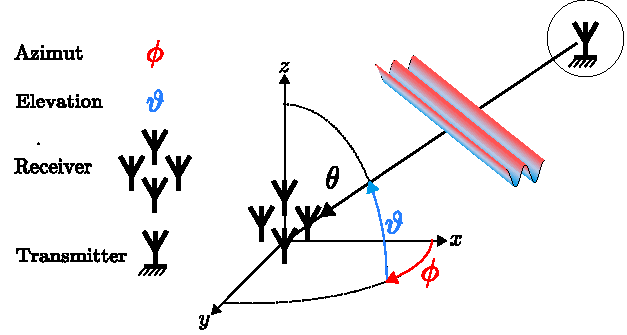
\includegraphics[width=0.6\textwidth]{figures/02_SignalModel/pointing_vect.drawio.pdf}
    \caption{Impinging wave-front - a visual representation of the Poynting vector \( \bfT \)}
    \label{fig:PointingVector}
\end{figure}
The x-axis of the cartesian coordinate system in \autoref{fig:PointingVector} is pointing towards the north, the
y-axis towards the east. Another simplifying assumption is the stationarity of the emitter during the duration of
one sampling period, which implies \( \frac{d\bfT}{dt} = 0 \).
\\

The emitter signal \( \widetilde{s}(t) \) can be expressed as a complex baseband signal \( s(t) \) modulated by a
carrier frequency \( f_C \)~\cite{tuncer.ch1}:
\begin{equation}
    \widetilde{s}(t) = s(t) \cdot \exp(j 2\pi f_C t)
    \label{eq:EmitterSignal}
\end{equation}
%---------------------------------------------------------------------------


\imgsection{Antenna Model}{figures/02_SignalModel/antenna.pdf}
\label{sec:AntennaModel}
The antenna model considers the directivity \( c(\theta, f_C) \) of real antennas which may distort the phase and
amplitude of received signals based on their frequency \( f_C \) and the angle of incidence \( \theta \).
The model assumes that the antenna is passive and does not amplify the received signal.
The voltage at the base of the antenna for an incoming wave is described in Equation~\eqref{eq:AntennaVoltage}.

\begin{equation}
    \widetilde{s}_A(t) = c(\theta, f_C) \cdot s(t) \cdot \exp(j 2\pi f_C t), \quad c \in \{c \in \mathbb{C} \,|\, |c| \leq 1\}
    \label{eq:AntennaVoltage}
\end{equation}
%---------------------------------------------------------------------------

\section{Measurement Model}
\label{sec:MeasurementModel}

\subsection{Introduction}
This section aims to elaborate on the measurement model used in the context of a \glsdesc{uca}.
A UCA comprises \( M \) antennas, uniformly distributed along a circle. The array enables the formation of an \( M \)-dimensional measurement
vector.
This measurement vector serves as the crucial link between the physical characteristics of incoming waves and the
digital signals that are subsequently processed.
The section further elaborates on how this model accommodates both single and multiple incoming waves.


\subsection{Single-Wave Case}
For a single incoming wave, each antenna \( A_m \) in an array of \( M \) antennas observes a phase \( \varphi_m \).
The phase differences \( \Delta\varphi_m \) between a reference antenna \( A_1 \) and all other antennas
\( A_m, \forall m \in \{2, 3, \ldots, M\} \) are expressed as:
\begin{align}
    \Delta\varphi_m(t) & = \varphi_m(t) - \varphi_1(t)                                                                                  \\
                       & = \pi \underbrace{\frac{d_{\text{Ant}}}{\lambda_C}}_D \cos(\elev) \sin\left(2\pi\frac{m-1}{M}-\azim\right).
    \label{eq:PhaseDiff}
\end{align}
The term \( \frac{d_{\text{Ant}}}{\lambda_C} \) is commonly denoted as aperture \( D \) and its influence on the array's
performance is discussed in Appendix~\ref{app:sec:ApertureInfluence}.\\
The narrowband approximation is a crucial assumption in~\eqref{eq:PhaseDiff}. It is expressed as
\( f_B \ll f_C \rightarrow d_{\text{Ant}}/\lambda_C \gg d_{\text{Ant}}/\lambda_B \), where \( f_B \) is the highest
occurring frequency in the baseband and \( f_C \) is the carrier frequency. This inequality implies that the phase
differences in the baseband signal are negligibly small compared to those at the carrier frequency.~\cite{tuncer.ch3}.

The relationship between the phase differences \( \Delta\varphi_m \) and the \gls{uca} are illustrated in \autoref{fig:UCA}.
\begin{figure}[H]
    \centering
    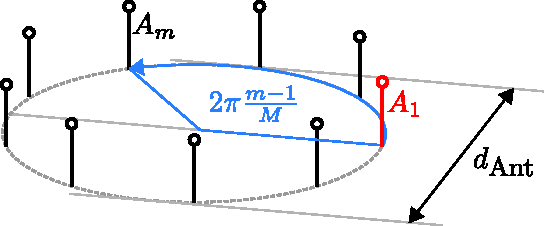
\includegraphics[width=0.5\textwidth]{figures/02_SignalModel/uca.pdf}
    \caption{The effect of the \gls{uca} on the phase differences \( \Delta\varphi_m \)~\cite{meyer}}.
    \label{fig:UCA}
\end{figure}

This leads to the antenna terminal voltage for the \( m \)-th antenna relative to the reference antenna as:
\begin{equation}
    \widetilde{s}_{A_m}(t) = c(\theta,f_C) \cdot \exp(j\Delta\varphi_m) \cdot \widetilde{s}(t)                \\
\end{equation}

The antenna terminal voltages are sampled and transformed into the complex baseband, introducing measurement noise. % TODO: Transformed to baseband. True?
This noise is assumed to be complex \gls{awgn} with zero mean and variance \( \sigma_\eta^2 \).
\( \eta_m \sim \mathcal{C}\mathcal{N}(0,\sigma_\eta^2) \), \( \eta_m \in \mathbb{C} \), and is statistically independent of the
baseband signal. The index \( k \) is defined as \( k = t / T_s \), where \( T_s \) is the sampling period.
This results in the measured voltage \( x_m[k] \) for the \( m \)-th antenna:
\begin{equation}
    x_m[k] = \underbrace{c(\bfT,\lambda_C) \cdot \exp(j\Delta\varphi_m)}_{a_m(\bfT)} \cdot s[k] + \eta_m[k]
    \label{eq:MeasScalar}
\end{equation}

The term \( a_m(\bfT) \) in~\eqref{eq:MeasScalar} is the \( m \)-th component of the steering vector \( \bfm{a}(\bfT) \),
which represents the array's spatial response to an impinging signal with from \( \bfT \), including amplitude
and phase information~\cite{oap.ch9}.
\begin{equation}
    \bfm{a}(\bfT) =
    \begin{bmatrix} a_1(\bfT) & a_2(\bfT) & \cdots & a_M(\bfT) \end{bmatrix}^T \in \mathbb{C}^{M}
    \label{eq:SteeringVector}
\end{equation}

Expanding~\eqref{eq:MeasScalar} to all \( M \) antennas yields the measurement vector \( \bfm{x}[k] \in \mathbb{C}^{M} \):
\begin{equation}
    \bfm{x}[k] = \bfm{a}(\bfT) \cdot s[k] + \bfm{\eta}[k],\quad \text{where}\: \bfm{\eta}[k] \sim \mathcal{C}\mathcal{N}(0,\sigma_\eta^2 \bfm{I}_M)
    \label{eq:MeasVecSingle}
\end{equation}

Considering the collection of all \( K \) measurements, results in the \textit{measurement matrix} \( \bfm{X} \)
\begin{equation}
    \bfm{X} = \begin{bmatrix} \bfm{x}[1] & \bfm{x}[2] & \cdots & \bfm{x}[K] \end{bmatrix} \in \mathbb{C}^{M \times K}
    \label{eq:MeasMatSingle}
\end{equation}
The measurement matrix \( \bfm{X} \) is commonly denoted as \( \bfm{x} \) -- measurement vector without the discrete time index.

The array manifold \( \mathfrak{A} \) is a function \( \mathfrak{A} : \mathbb{R}^2 \to \mathbb{C}^{M} \) that transforms
unit amplitude signals from spatial directions \( \bfT \in \mathbb{R}^2 \) into steering vectors
\( \bfm{a}(\bfT) \in \mathbb{C}^{M} \)~\cite{oap.ch4, tuncer.ch1}. Essentially, it characterizes the array's spatial
response to an incoming unit amplitude signal for given spatial parameters \( \bfT \)~\cite{yu22RCNN}.

\begin{figure}[H]
    \centering
    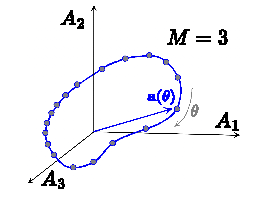
\includegraphics[width=0.6\textwidth]{figures/02_SignalModel/array_manifold.pdf}
    \caption{The array manifold \( \mathfrak{A} \)~\cite[ch4.5.2]{demmel}}
    \label{fig:ArrayManifold}
\end{figure}

\autoref{fig:ArrayManifold} visually represents the array manifold \( \mathfrak{A} \) by displaying the locus of
steering vectors for an antenna array with \( M = 3 \) antennas.
\\

\subsubsection*{Multi-Wave Scenario}
In scenarios involving multiple incoming waves, let \( \Theta = \{\bfT_1, \ldots, \bfT_N\} \) represent the set of
directions of theses \( N \)%
\footnote{The number of impinging waves \( N \) is also referred to as the \textbf{model order}.}
impinging waves. The Steering Matrix \( \bfm{A} \) is then defined as the set of steering vectors
corresponding to this \( \Theta \). The matrix has dimensions \( M \times N \) and is expressed as:
\begin{align}
    \bfm{A}(\bfm{\Theta}) =
    \begin{bmatrix} \bfm{a}(\bfT_1) & \cdots & \bfm{a}(\bfT_N) \end{bmatrix}
    \label{eq:SteeringMatrix}
\end{align}
Hence, the measurement vector in this multi-wave scenario becomes:
\begin{align}
    \bfm{x}[k] = \bfm{A}(\bfm{\Theta}) \bfm{s}[k] + \bfm{\eta}[k].
    \label{eq:MeasVecMult}
\end{align}

% \subsubsection*{Discrete Approximation of the Array Manifold}

% Immediately following our discussion on the continuous array manifold \( \mathfrak{A} \), it is pertinent to introduce
% its discrete approximation \( \widehat{\mathfrak{A}} \). This approximation is constructed from a finite set
% \( \{\bfT_1', \ldots, \bfT_Q'\} \) of spatial directions and serves as a sampled representation of \( \mathfrak{A} \).
% It is defined as:
% \begin{align}
%     \widehat{\mathfrak{A}} =
%     \begin{bmatrix}
%         a_1(\bfT_1') & \cdots & a_1(\bfT_Q') \\
%         \vdots       & \ddots & \vdots       \\
%         a_M(\bfT_1') & \cdots & a_M(\bfT_Q')
%     \end{bmatrix},
%     \quad \widehat{\mathfrak{A}} \in \mathbb{C}^{M \times Q}.
% \end{align}
% This discrete approximation will be essential for subsequent computational applications, such as the \gls{music} algorithm.




\section{Covariance Matrix and Subspaces}
\label{sec:CovarianceMatrix}
In the realm of advanced signal processing, covariance matrices serve as a cornerstone, particularly for
super-resolution \gls{doa} techniques such as \gls{music}, detailed in~\autoref{ch:OverviewMUSIC}. These techniques rely
on the evaluation of the subspaces spanned by the eigenvectors derived from the covariance matrix.
On the other hand, \gls{moe} methods, discussed in~\autoref{ch:ModelOrderEstimation}, as well as the Deep Learning (DL) approaches
examined in this thesis, focus primarily on the eigenvalues of the covariance matrix. This section delves into the
mathematical foundations of the covariance matrix, elucidates its significance in the derivation of signal and noise
subspaces, and outlines the conditions required for its accurate estimation in real-world applications.


\subsection{Subspaces}
\label{sec:sub:subspaces}
The notion of signal and noise subspaces is pivotal in the field of \gls{doa} estimation, especially when employing
super-resolution algorithms such as \gls{music}, as elaborated in~\autoref{ch:OverviewMUSIC}.
In mathematical terms, the signal subspace represents the span of measurement vectors \( \bfm{x}_i[k] \) in complex
space \( \mathbb{C}^M \) for a given \( \bfT_i \). This span can also be understood as a subset of points in
\( \mathbb{C}^M \) reachable by the linear combinations of the measurement vectors. Thus, the signal subspace
\( \bfm{U}_S \) is formally defined as:
\begin{equation}
    \bfm{U}_S = \mathrm{span}\{\bfm{x}_i[k]\} \subseteq \mathbb{C}^M
\end{equation}
The concept of the signal subspace provides an intuitive geometric representation of the measurement vectors as
previously described in~\autoref{sec:MeasurementModel}, given \( M = 3 \) antennas in three-dimensional space.
For a single-wave scenario, the noiseless measurement vector, \( \bfm{x}_i[k] \), manifests as a finite line
passing through the origin in \( \mathbb{C}^M \), characterized by its direction vector \( \bfm{a}(\bfT) \)~\cite{meyer}.
In a multi-wave context, each measurement vector \( \bfm{x}_i[k] \) can be considered a linear combination of
vectors \( \bfm{a}(\bfT_n) \). These vectors span the signal subspace \( \bfm{U}_S \), which is mathematically
defined as \( \bfm{x}_i[k] \in \bfm{U}_S \subseteq \mathbb{C}^M \)~\cite{meyer}. Both abovementioned scenarios
are illustrated in~\autoref{fig:subspace}.

\begin{figure}[H]
    \centering
    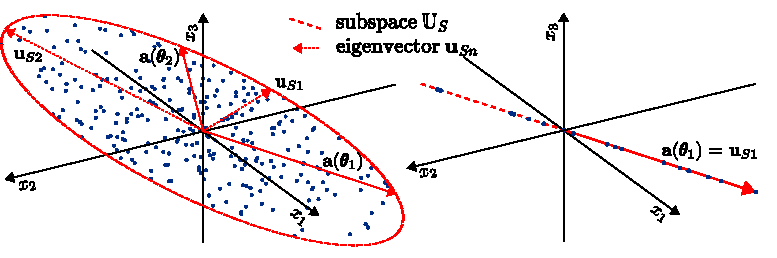
\includegraphics[width=0.9\textwidth]{figures/02_SignalModel/subspace.pdf}
    \caption{The signal subspace \( \bfm{U}_S \) for two and a single impinging wave(s)~\cite{meyer}}
    \label{fig:subspace}
\end{figure}

As per \autoref{eq:MeasVec}, additive white Gaussian noise \( \bfm{\eta}[k] \sim \mathcal{C}\mathcal{N}(0,\sigma_\eta^2\bfm{I}) \)
superimposes the linear combinations of steering vectors \( \bfm{a}(\bfT_n) \).
Given the presence of \( N \) waves, which span an \( N \)-dimensional signal subspace \( \bfm{U}_S \),
the noise subspace \( \bfm{U}_\eta \) spans an \( M \)-dimensional sphere in \( \mathbb{C}^M \).

Both subspaces are characterized by their eigenvectors \( \bfm{U} \) and eigenvalues \( \bfL \).
\begin{align}
    \bfm{C} & = \sum_{m=1}^M \lambda_m \bfm{u}_m \bfm{u}_m^H                                                 \\
            & = \bfm{U}_S \bfm{\Lambda}_S \bfm{U}_S^H + \bfm{U}_{\eta} \bfm{\Lambda}_{\eta} \bfm{U}_{\eta}^H
    \label{eq:EigenvalueDecomposition1}
\end{align}
In \autoref{eq:EigenvalueDecomposition1}, the eigenvalues
\( \bfm{\Lambda} = \text{diag}\{\lambda_1, \lambda_2, \ldots, \lambda_N\} \) and their corresponding eigenvectors
\( \bfm{U} = [\bfm{u}_{1},\ldots,\bfm{u}_{N}] \) are sorted in descending order, that is,
\( \lambda_1 \geq \lambda_2 \geq \cdots \geq \lambda_N \), as described in~\cite{tuncer.ch5}.

The signal subspace \( \bfm{U}_S \) is spanned by the first \( N \) eigenvectors,
\( \bfm{U}_S = [\bfm{u}_{1},\ldots,\bfm{u}_{N}] \), corresponding to the largest \( N \) eigenvalues.
Conversely, the noise subspace \( \bfm{U}_{\eta} \) is spanned by the remaining eigenvectors
\( \bfm{U}_{\eta} = [\bfm{u}_{N+1}, \ldots, \bfm{u}_{M}] \), which correspond to the smaller eigenvalues.

% \begin{equation*}
%     \bfm{U} &= \begin{bmatrix} \bfm{u}_{1} & \cdots & \bfm{u}_{N} & \bfm{u}_{N+1} & \cdots & \bfm{u}_{M} \end{bmatrix}
% \end{equation*}

\subsection{Covariance Matrix and its Eigenvalue Decomposition}
Expanding on the foundational principles of signal and noise subspaces, the covariance matrix \( \bfm{C} \) plays an
indispensable role in eigenvalue-based methods for \gls{doa} and \gls{moe} estimation. The covariance matrix captures
the second-order statistics of the received signals\footnote{Refer to \autoref{app:sec:GeneralCovMatrix} for a
    comprehensive form of the covariance matrix}, thereby integrating both their signal and noise attributes.

The covariance matrix \( \bfm{C} \) was previously introduced in \autoref{eq:EigenvalueDecomposition1}, constructed
from the eigenvalues \( \bfm{\Lambda} \) and eigenvectors \( \bfm{U} \) that characterize the signal and noise
subspaces. Given that these characteristics are not known a priori and are essentially the information sought for
\gls{doa} and \gls{moe} estimation, alternative methods must be employed for constructing the covariance matrix to
then being able to perform an eigenvalue decomposition.

If the signal and noise vectors are zero mean, and if the noise is spatially white and statistically independent of the
source signals~\cite{tuncer.ch5}, then the \( M \times M \) array covariance matrix can be calculated as:
\begin{align}
    \bfm{C}_x & = \mathbb{E}[\bfm{x}[k] \bfm{x}^H[k]]  \label{eq:CovarianceExpanded1}                                                                                                                                                                   \\
              & = \bfm{A} \mathbb{E}[\bfm{s}[k] \bfm{s}^H[k]] \bfm{A}^H + \bfm{A} \mathbb{E}[\bfm{s}[k] \bfm{\eta}^H[k]] + \mathbb{E}[\bfm{\eta}[k] \bfm{s}^H[k]] \bfm{A}^H + \mathbb{E}[\bfm{\eta}[k] \bfm{\eta}^H[k]]  \label{eq:CovarianceExpanded2} \\
              & = \underbrace{\bfm{A} \mathbb{E}[\bfm{s}[k] \bfm{s}^H[k]] \bfm{A}^H}_{\bfm{C}_S} + \; {\color{red}{0}} \; + \underbrace{\sigma_\eta^2 \bfm{I}}_{\bfm{C}_\eta} \label{eq:CovarianceExpanded3}                                                 \\
              & = \bfm{C}_S + \sigma_\eta^2 \bfm{I}  \label{eq:CovarianceExpanded4}
\end{align}\cite[Chapter 4]{meyer}

As shown in~\eqref{eq:CovarianceExpanded2}, the measurement vector \( \bfm{x} \) is decomposed into its signal component
\( \bfm{s} \), transformed by the steering matrix \( \bfm{A}(\bfm{\Theta}) \), and additive noise \( \bfm{\eta} \),
based on \autoref{eq:MeasVecMult}.
The terms related to cross-correlation in~\eqref{eq:CovarianceExpanded2} become zero, given the assumption that the
signal and noise are zero-mean and uncorrelated. This simplification leads to the final form of the covariance matrix
as shown in~\eqref{eq:CovarianceExpanded4}.
The noise covariance matrix \( \bfm{C}_\eta \) is denoted as \(\sigma_\eta^2 \bfm{I}\), where \(\sigma_\eta^2\) is the noise variance. Similarly,
\( \bfm{C}_S \) represents the signal covariance matrix.


\subsubsection*{Estimation of the Covariance Matrix}
In real-world scenarios, the covariance matrix \( \bfm{C}_x \) is typically estimated from a finite set of snapshots
\( K \) of the measurement vector \( \bfm{x}[k] \). The maximum-likelihood estimate for \( \bfm{C}_x \) is given by:
\begin{equation}
    \C = \frac{1}{K} \sum_{k=1}^{K} \bfm{x}[k] \bfm{x}^H[k]
    \label{eq:SampledCovarianceMatrix}
\end{equation}
The fidelity of the covariance matrix approximation improves as the number of snapshots \( K \) increases,
asymptotically approaching the true covariance matrix as \( K \to \infty \)~\cite{tuncer.ch7}.\\
All quantities derived from the estimated covariance matrix are denoted as follows%
\footnote{The model order \( N \), through its own merit, has earned the privilege of wearing a hat when estimated.}
\begin{align*}
    \bfm{U} & \mapsto \widehat{\bfm{U}} \\
    \bfm{U}_S & \mapsto \UsH \\
    \bfm{U}_{\eta} & \mapsto \UnH \\
    \bfL & \mapsto \widehat{\bfL} \\
\end{align*}


It is essential to have more samples \( K \) than antennas \( M \) for a reliable covariance matrix approximation.
This requirement ensures that each distinct eigenvalue of the true covariance matrix corresponds to a unique cluster in
the eigenvalue distribution. A sufficient number of samples allows for the separation of these clusters, enabling
accurate estimation of eigenvalues and eigenvectors, and thereby reducing ambiguity and enhancing the approximation's
accuracy~\cite{tuncer.ch7}.



\subsubsection*{Eigenvalue Decomposition of the Covariance Matrix}
The covariance matrix \( \bfm{C}_x \) is a Gram matrix and is positive semi-definite, a trait ensuring that its
eigenvalues are real and non-negative~\cite{tuncer.ch4}.

\begin{align}
    \bfL & = \sigma_\eta^2 + \bfL_S                                                                                                  \\
                  & = \begin{bmatrix} \lambda_{S_1} + \sigma_\eta^2 & \cdots & \lambda_{S_N} + \sigma_\eta^2 & \sigma_\eta^2 & \cdots & \sigma_\eta^2 \end{bmatrix}^T
    \label{eq:eigval_superimposed}
\end{align}\cite{oap.ch5, meyer}

All eigenvalues are superimposed by the noise variance \( \sigma_\eta^2 \), causing the covariance matrix to become positive
finite~\cite{tuncer.ch4, oap.ch5}. \\
Each noise eigenvalue \( \lambda_i \in \bfL_{\eta}\) for \( i \in \{N, \ldots, M\} \) is normally distributed \( \lambda_i \sim \mathcal{N}(\sigma^2_{\eta}, 0) \)
with mean \( \sigma^2_{\eta} \) and variance 0.

When \( \widehat{\bfL} \) is considered for a finite number of snapshots, the
noise eigenvalues \( \lambda_i \in \bfL_{\eta}\) for \( i \in \{N, \ldots, M\} \) empirically appear to be drawn from independent normal distributions
whose means are less than \( \sigma^2_{\eta} \) and separated approximately uniformly.
These distributions converge asymptotically to the theoretical value as \( K \to \infty \).
\begin{equation}
    \mathcal{N}(\mathbb{E}[\lambda_{i, \eta}], \sigma^2_{\lambda_{i, \eta}}) \stackrel{K \rightarrow \infty}{\xrightarrow{\hspace*{1cm}}} \mathcal{N}(\sigma^2_{\eta}, 0), \quad i \in \{N, \ldots, M\}
\end{equation}

\section{Incoherent Measurement Model}
\label{sec:InherentMeasurementModel}

The incoherent measurement model represents an adaptation of the coherent measurement framework, previously established,
to situations where the number of available antenna paths \( L \) is fewer than the total number of antennas \( M \).
This adaptation is necessitated by resource constraints inherent to each antenna path%
\footnote{Tuners, analog filters, ADCs, DDCs, ...\cite{demmel}.},
that limit the number of paths that can be simultaneously processed.
Considering a scenario with 9 antennas and 3 antenna paths, one path is permanently allocated to the reference antenna,
while the other two are switched in time-division across the remaining antennas.

\subsection{Incoherent Measurement Vector}
\label{subsec:IncoherentMeasurementVector}
The incoherent measurement vector \( \bfm{x}'[k] \) is an extension of the coherent measurement vector introduced
in \autoref{eq:MeasVec} for cases when \( L < M \). It captures the signal from a subset of antennas at each snapshot
and is formulated as follows~\cite[Chapter 6]{meyer}:
\begin{align}
    \bfm{x}'[k] &= \bfm{D}[j] \bfm{x}[k], & \bfm{x}' \in \mathbb{C}^{M} \\
    j &= \text{mod}(k-1, J) + 1.
\end{align}
Here, \( k \) represents the snapshot index, and \( j \) indicates the specific switching step within a cycle determined
by the total number of steps \( J \) -- \( J \) being the number of subarrays. This model assumes a time-division strategy, where different subsets of antennas
are activated at different times to form the overall measurement.%

\begin{table}[H]
    \caption{Sampling cycle for a \gls{uca} with \( M = 9 \) antennas and \( L = 3 \) RF-paths.}
    \label{tab:SamplingCycle}
    \centering
    \begin{tabular}{>{\bfseries}c*{5}{c}}
      \toprule
      Antenna Base & Path 1-2 & Path 1-3 & Path 2-3 & Diagonal & DF1 DF2 DF3 \\
      \midrule
      1 & \(x_{12}\) & \(x_{19}\) & \(x_{29}\) & \(\varnothing\) & \(A_{1}\, A_{2}\, A_{9}\) \\
      2 & \(x_{13}\) & \(x_{18}\) & \(x_{38}\) & \(\varnothing\) & \(A_{1}\, A_{3}\, A_{8}\) \\
      3 & \(x_{14}\) & \(x_{17}\) & \(x_{47}\) & \(\varnothing\) & \(A_{1}\, A_{4}\, A_{7}\) \\
      4 & \(x_{15}\) & \(x_{16}\) & \(x_{56}\) & \(x_{11}\) & \(A_{1}\, A_{5}\, A_{6}\)  \\
      \vdots & \vdots & \vdots & \vdots & \vdots & \vdots \\
      12 & \(x_{78}\) & \(x_{79}\) & \(x_{89}\) & \(x_{88}\) & \(A_{7}\, A_{8}\, A_{9}\) \\
      \bottomrule
    \end{tabular}
  \end{table}


\subsection{Impact on the Estimated Covariance Matrix}
\label{subsec:ImpactOnTheCovarianceMatrix}
Subsampling in an incoherent measurement setup negatively affects the estimation of the covariance matrix, \( \Csub \), as it's
based on a subset of the full antenna array signals at each snapshot. This leads to a covariance matrix that may not
fully capture the true signal correlations, denoted as:
\begin{equation}
    \Csub = \frac{1}{KJ}\sum_{\substack{k=1 \\ j=\text{mod}(k-1, J) + 1}}^{KJ} \text{selDiag} \left(\bfm{D}[j] \bfm{x}[k] \bfm{x}^H[k] \bfm{D}^H[j] \right)
    \label{eq:sub_sampled_covmat}
\end{equation}

The function ``selDiag'' selects the diagonal elements of the sub-array covariance matrices according to the switching
scheme outlined in \autoref{tab:SamplingCycle}. This process is essential to ensure that the diagonal elements of the
covariance matrices are sampled only once per antenna cycle. While the discarding of most off-diagonal elements certainly
results in a loss of information, the employment of according scaling factors to compensate for the varied accumulation
frequencies of the principal and off-diagonal elements has been shown to result in numerical errors.
As a result of the degraded estimation of the covariance matrix, the eigenvalues derived from \( \Csub \) exhibit
increased variance and potentially negative values.
The situation is further exacerbated when the number of snapshots is low, as more samples are generally required to achieve
an accurate estimation of the true covariance matrix.
This corruption of the eigenvalues leads to various challenges with typically employed \gls{doa} estimation techniques,
and exacerbates the problem of model order selection~\cite[Chapter 6, 8]{meyer}.

While the incoherent measurement vector and the respective sub-sampled covariance matrix will be the basis for all following sections, we will no longer distinguish
between coherent and incoherent values or symbols throughout the rest of this thesis for sake of convenience.


\section{Conclusion}
\label{sec:Conclusion}

\begin{figure}[H]
    \centering
    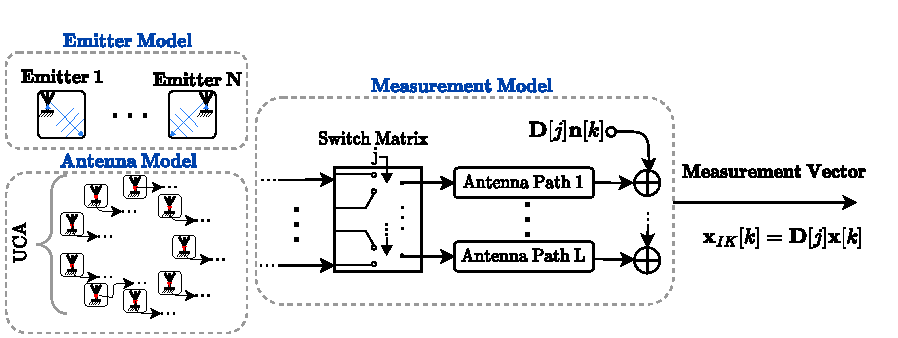
\includegraphics[width=1\textwidth]{figures/02_SignalModel/meas_model.pdf}
    \caption{The incoherent measurement model}
    \label{fig:IncoherentMeasurementModel}
\end{figure}

The data model as illustrated in \autoref{fig:IncoherentMeasurementModel} showcases the interplay of the various
``sub-models'' explored in this chapter. Starting with the emitter model, which assumed the far-field propagation of
a narrowband signal, followed by the antenna model, which considered the directivity of real antennas, and finally
the measurement model (\autoref{sec:MeasurementModel}), which captured the spatial relationship of the received
fields to the antenna array. The measurement model depicted in \autoref{fig:IncoherentMeasurementModel}, shows the
extension of the coherent measurement model, which was explored in the previous section.


\endinput




